\section{Large Language Models}

When we talk about Large Language Models (LLMs), we refer to advanced software designed to communicate in a human-like manner. These models possess the remarkable ability to understand complex contexts and generate consistent, human-like content. If you have ever interacted with a chatbot or AI virtual assistant, you may have used an LLM without realizing it. LLMs are used in various applications such as text generation, machine translation, sentiment analysis and document summarization, among others. They have become an essential part of the artificial intelligence (AI) landscape. This section delves into their history and evolution, including an analysis of the architecture of the transformer.

LLMs refer to large, general-purpose language processing models that are pre-trained on large datasets to learn the fundamental structures and semantics of human language. The term “large” indicates both the significant amount of data needed for training and the billions or even trillions of parameters these models contain. Pre-training enables LLMs to handle common language tasks such as text classification, question answering and document summarization. After pre-training, these models are typically fine-tuned to smaller, specialized datasets for specific domains, improving their accuracy and efficiency. \cite{researchgraph2024}

\subsection{Evolution of Large Language Models}

\subsubsection{Early Days: Chatbots and Rule-Based Systems (1960s)}

The journey of LLMs began in the 1960s with ELIZA, an early natural language processing computer program created by Joseph Weizenbaum \cite{weizenbaum1966eliza}. ELIZA was able to simulate a conversation by searching for key words and using programmed responses. Following ELIZA, SHRDLU, developed by Terry Winograd in the early 1970s \cite{winograd1972understanding}, was an advanced program capable of understanding and manipulating a virtual block world through natural language commands. This marked a significant step toward machine understanding of context and intentions.

\begin{figure}[h!]
    \centering
    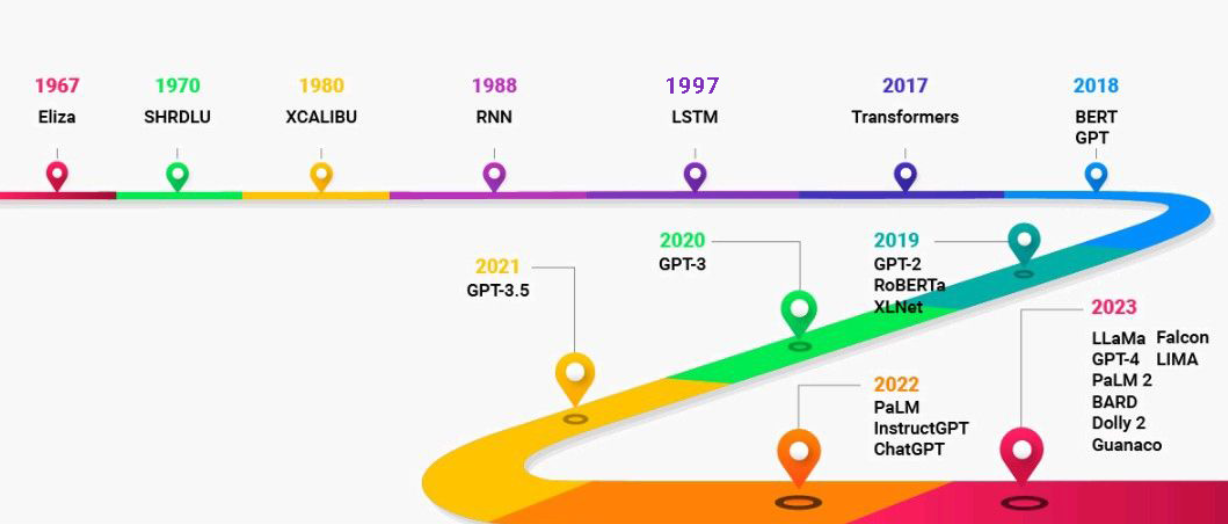
\includegraphics[width=0.6\textwidth]{images/llms/llms-history.png}
    \caption{Timeline of Large Language Models (LLMs) development. \textit{Source:} \cite{AnalyticsVidhya2023}}
    \label{fig:llms-history}
\end{figure}

\subsubsection{Rise of Recurrent Neural Networks (1980s)}

In the late 20th century, recurrent neural networks (RNNs), inspired by the interconnected neurons of the human brain, were born. Introduced in 1986, RNNs gained popularity for their ability to remember previous inputs and process sequential data, making them suitable for NLP tasks. However, RNNs have had limitations with long sentences, often suffering from the gradient vanishing problem \cite{elman1990finding}.

\subsubsection{Rise of Long Short-Term Memory (1990s)}

Long short-term memory (LSTM), a specialized type of RNNs, was introduced in 1997 to address the limitations of RNNs. LSTMs are capable of remembering information over long sequences, overcoming the short-term memory limitations of RNNs. Their unique architecture, with input, forgetting, and output gates, allowed LSTMs to retain relevant information in memory, making them more efficient for capturing long-term dependencies in sentences \cite{hochreiter1997long}.

\subsubsection{Gated Recurrent Units (2010s)}

In 2014, Gated Recurrent Units (GRUs) were introduced to solve problems similar to LSTMs, but with a simpler structure. GRUs use only two ports: an update port and a reset port, making them more computationally efficient, while maintaining the long-term dependencies in the sentences \cite{cho2014learning}.

\subsubsection{Rise of Attention Mechanism (2014)}

The introduction of the attention mechanism on paper on neural machine translation \cite{bahdanau2014neural} in 2014 marked a paradigm shift in sequence modeling. Unlike RNNs, which process sentences with a context vector of fixed size, attention mechanisms allowed models to dynamically select relevant parts of the source sequence, ensuring that crucial information was not lost, especially in longer sequences.

\subsubsection{The Invention of Transformers Architecture (2017)}

Transformers, introduced in 2017 by Vaswani et al. in the paper “Attention is All You Need” \cite{vaswani2017attention}, relied on an attention mechanism to process sequences. The processors featured an encoder-decoder architecture with multiple layers of self-attention and feed-forward neural networks. The multi-layered attention mechanism allowed the processors to simultaneously focus on different parts of the input sentence, capturing various contextual nuances. Processors could also process sequences in parallel, rather than sequentially, leading to the development of sophisticated LLMs such as BERT and GPT. Given its importance and influence in the AI field, the transformer architecture will be discussed in more depth in later sections.

\subsubsection{Emergence of Large Language Models (2018-Onwards)}

With the success of transformers, scaling these models became the next logical step. Google's BERT model, released in 2018, processed text bidirectionally, setting new performance standards in various benchmarks \cite{devlin2018bert}. OpenAI's GPT-2, released in 2019, and GPT-3 in 2020, demonstrated the capabilities of generative models in performing a wide range of tasks \cite{radford2019language}. OpenAI continued to advance the GPT series with GPT-3.5 in 2022, GPT-4 in 2023 and GPT-4o in 2024. ChatGPT, based on GPT-3.5, became the fastest growing consumer application in history after its release in November 2022.

Other major players in the technology industry and academia have also contributed to the development of LLMs. Google's PaLM (Pathways Language Model) was released in March 2023, followed by PaLM 2 in May 2023 \cite{chowdhery2023palm}. In December 2023, Google unveiled Gemini, a multimodal model capable of processing different forms of information. Meta AI released the LLaMA (Large Language Model Meta AI) series in 2023, offering open-source models for research and commercial use \cite{touvron2023llama}. Anthropic introduced the Claude series in 2023, prioritizing the universal benefits and security of AI \cite{anthropic2024claude}. \newline

The evolution of language models from simple rule-based systems to complex intelligence models means significant progress in artificial intelligence technology. Today, LLMs are more than just tools for improving text-based applications; they are increasingly capable of understanding and communicating with humans. Moreover, multimodal LLMs are able to handle not only text, but also images, sounds and videos, integrating various forms of data to comprehensively understand and analyze different contexts. These models are transforming the way we interact with technology, making it more accessible and responsive to human needs. In essence, LLMs are becoming powerful partners for humans, helping us tackle multiple tasks and simplifying our lives in various ways. \cite{researchgraph2024}

\section{Transformer Architecture}

As highlighted in the previous section, a key breakthrough in language modeling, central to all modern state-of-the-art LLMs, was the introduction of transform architecture and the self-attention mechanism in 2017. This advance was presented in the seminal paper “Attention is All You Need” by Vaswani et al. \cite{vaswani2017attention}, which revolutionized natural language processing (NLP) by enabling models to capture long-range dependencies much more efficiently than previous architectures.

\begin{figure}[h!]
    \centering
    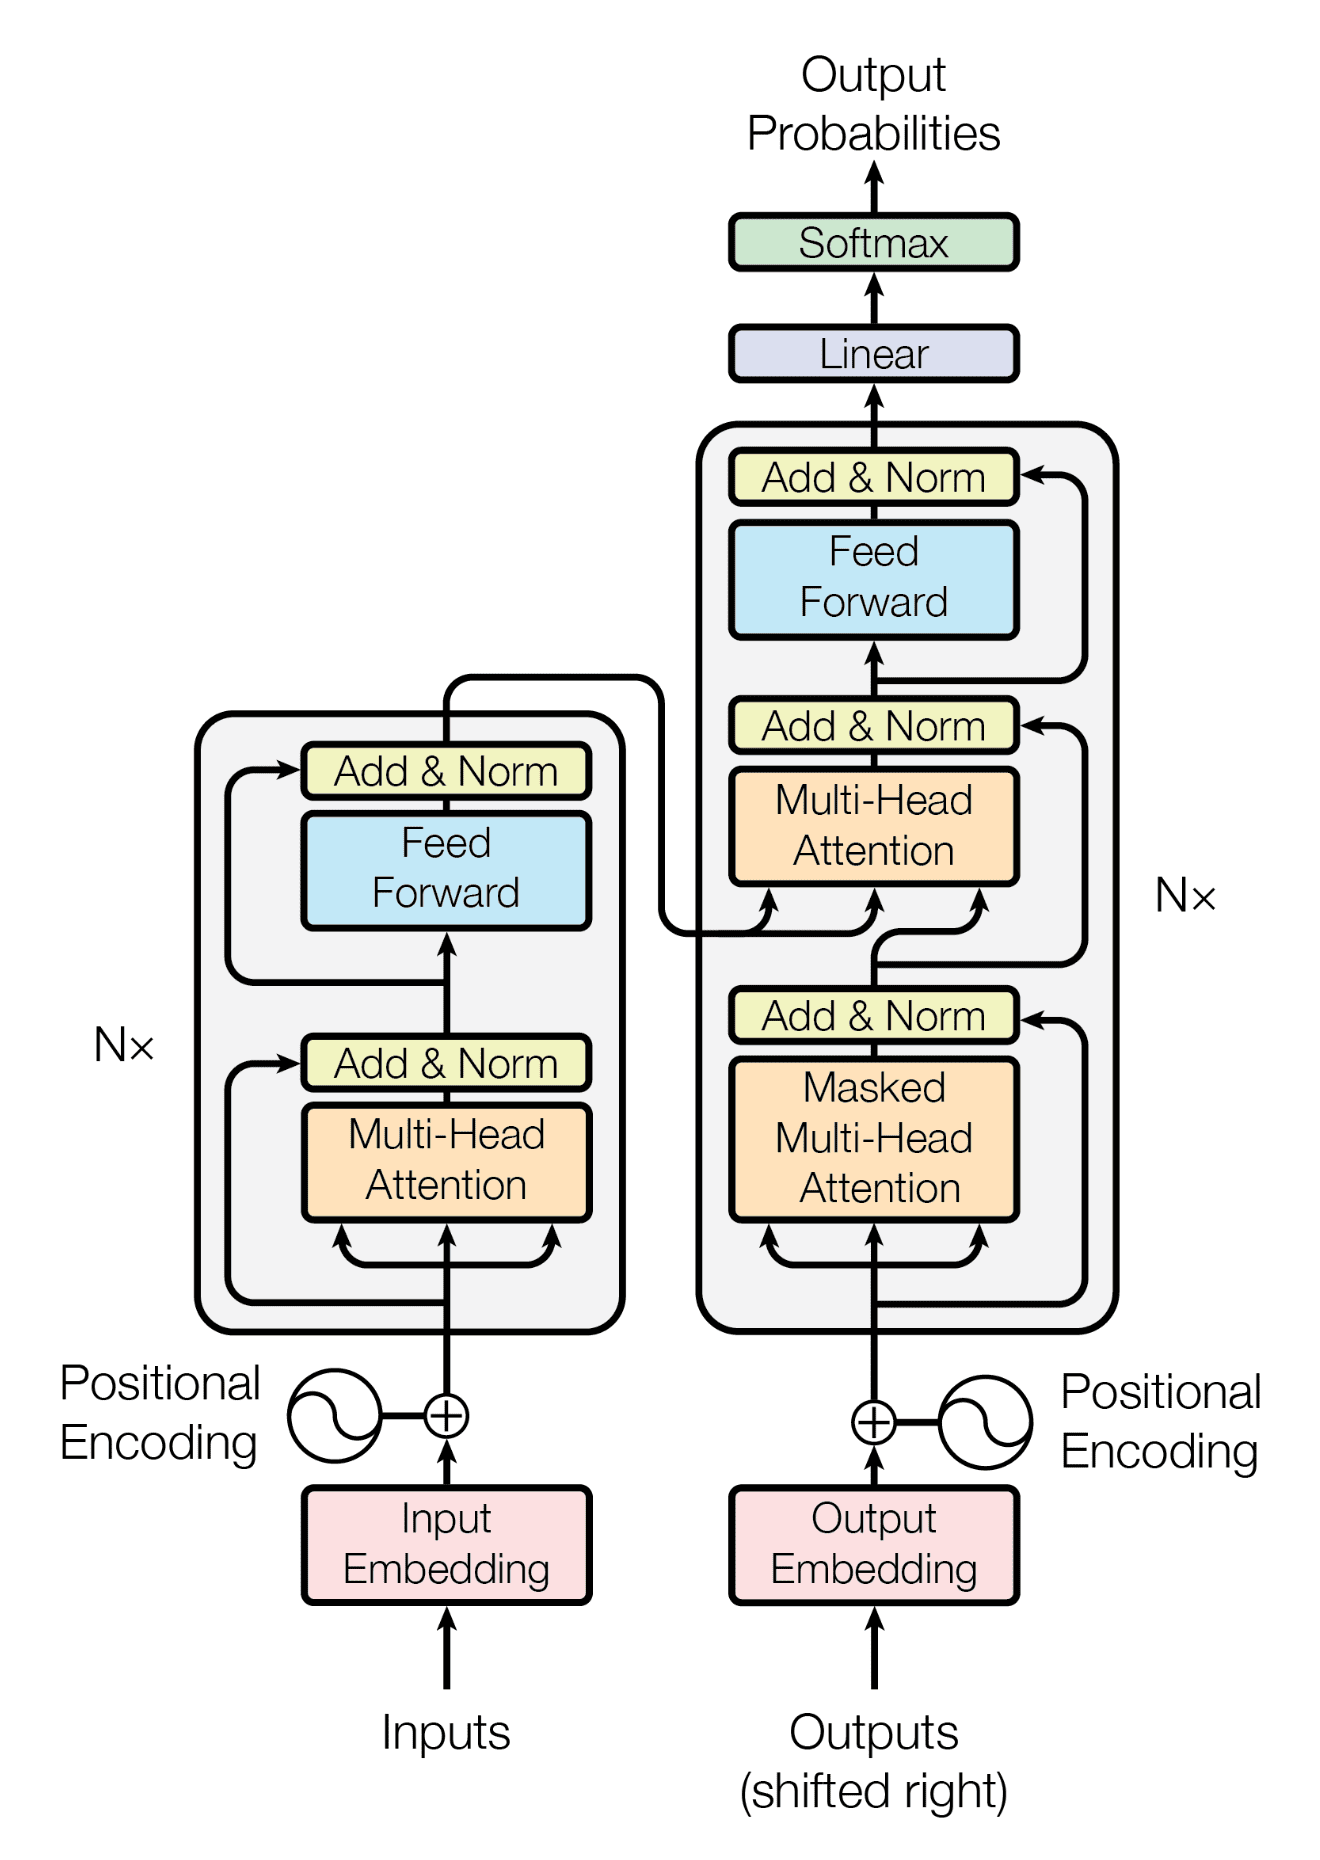
\includegraphics[width=0.6\textwidth]{images/llms/transformer-architecture.png}
    \caption{The general architecture of the transformer, composed of an encoder and a decoder. The encoder takes the input sequence and converts it into continuous representations, while the decoder generates the output sequence from these representations. \textit{Source:} \cite{vaswani2017attention}}
    \label{fig:transformer-architecture}
\end{figure}

The self-attention mechanism is a key component of the transformer, enabling models to weigh the importance of different elements in a sequence by measuring the similarity between elements and determining the amount of attention each element should pay to the others. This mechanism enables the model to grasp complex relationships and dependencies in the entire input sequence, enhancing its ability to understand and generate coherent, context-aware outputs. In NLP, the self-attention mechanism effectively models the relationships between all words in a sentence, facilitating better understanding and generation of text.

The great advantage of the transformer architecture of being highly parallelizable makes it computationally efficient and able to handle input sequences of varying lengths. The ability to process all elements of a sequence simultaneously, rather than sequentially, significantly reduces training time for large data sets. This parallelism, combined with the effectiveness of the self-attention mechanism, has made the transformer the basis for state-of-the-art models in machine translation, text generation and many other NLP tasks.

As illustrated in Figure \ref{fig:transformer-architecture}, the overall transformer architecture consists of an encoder and a decoder, with each component playing a crucial role in processing and sequence generation. The transformative impact of this architecture continues to drive advances in NLP and AI. The key elements of this architecture, such as positional encoding, multi-headed attention, feed-forward neural networks, norm step addition, residual connections, layer normalization, and linear and softmax final layers, will be discussed in the subsequent sections to provide a more detailed understanding of these components.

\subsubsection{Positional Encoding}

In the field of natural language processing (NLP), transformer models have radically changed our approach to sequence-sequence tasks. Unlike traditional recurrent neural networks (RNNs) or convolutional neural networks (CNNs), transformers process tokens in parallel and have no intrinsic awareness of token order. Positional encodings are a key technique for incorporating transformer models with an understanding of sequence order, enabling them to effectively process and understand input sequences. \cite{li2023transformer}

Positional encodings play a key role in transformer models for several reasons:

\begin{itemize}
    \item \textbf{Preserve sequence order:} Transformer models handle tokens in parallel and have no intrinsic information about token order. Positional encodings provide this information, allowing the model to distinguish tokens based on their position. This is essential for tasks where word order is important, such as language translation and text generation.
    
    \item \textbf{Maintaining Contextual Information:} In NLP tasks, the meaning of a word often depends on its position within the sentence. For example, the word “cat” in “The cat sat on the carpet” has a different meaning than “The carpet sat on the cat.” Positional encodings help maintain this contextual information, allowing the model to understand the correct meaning based on word order.
    
    \item \textbf{Improving generalization}. By incorporating positional information, transformer models can better generalize between sequences of different lengths. This is especially important for tasks where the length of the input sequence varies, such as summarizing documents or answering questions. Positional encodings allow the model to handle input sequences of different lengths without compromising performance.
    
    \item \textbf{Mitigate symmetry:} Without positional encodings, the self-attention mechanism of transformational models treats tokens symmetrically, which can lead to ambiguous representations. Positional encodings introduce asymmetry, ensuring that tokens in different positions are treated distinctly, thus improving the model's ability to capture long-range dependencies \cite{geeksforgeeks2024-pe}.
\end{itemize}

The original transformer paper by Vaswani et al. \cite{vaswani2017attention} introduced sinusoidal positional encodings. The idea is to produce unique encodings for each position that can be added to token embeddings, allowing the model to distinguish the position of each token in a sequence. For position \( p \) and size \( i \), the positional encoding is calculated as:
\begin{equation}
    PE(p, 2i) = \sin\left(\frac{p}{10000^{2i/d}}\right)
\end{equation}

\begin{equation}
    PE(p, 2i + 1) = \cos\left(\frac{p}{10000^{2i/d}}\right)
\end{equation}

where \( d \) is the dimensionality of embeddings. These sinusoidal functions ensure that positional encodings are unique and can convey position-related information that can be used by attention mechanisms. Each dimension of the positional encoding aligns with a sine or cosine function of different wavelengths, creating a geometric progression from \( 2\pi \) to \( 10000 \times 2\pi \). For any fixed offset \( k \), \( PE(p+k) \) can be expressed as a linear function of \( PE(p) \).

Kazemnejad \cite{kazemnejad2019:pencoding} provides an intuitive explanation of this encoding scheme, emphasizing its ability to capture positional information in a way that satisfies several important criteria: it must produce a unique encoding for each time-step, maintain consistent distances between time-steps in sentences of different lengths, generalize to longer sentences, and remain deterministic.

In more recent large language models (LLMs), positional encoding often uses learned rather than sinusoidal encodings. In this approach, positional encodings are randomly initialized model parameters learned during training, similar to token encodings. The size of the learned positional encoding vector is related to the maximum sequence length that the model can handle. For example, the BERT model \cite{devlin2018bert} employs a positional encoding size of \( 768 \times 512 \), limiting BERT to a maximum input length of 512 tokens. Although the fixed maximum input length is a disadvantage of learned positional encodings, they can adapt during training, allowing the model to learn positional representations better suited to the training data, unlike static sinusoidal encodings.

\subsubsection{Self-attention mechanism}

The self-attention mechanism is a key component of the transformer architecture, enabling the model to dynamically evaluate the relative importance of different words in a sequence. Initially introduced in the seminal article “Attention is All You Need” by Vaswani et al. \cite{vaswani2017attention}, self-attention is essential for understanding the context and relationships between words, thus enhancing the model's ability to capture long-range dependencies.

In the self-attention mechanism, each token of an input sequence \( X \) with tokens \( x_1, x_2, \ldots, x_n \) is transformed into three vectors:
\begin{itemize}
    \item \textbf{Query (Q):} It represents the token in question.
    \item \textbf{Key (K):} Represents all tokens against which the query is compared.
    \item \textbf{Value (V):} Contains the information of the tokens.
\end{itemize}

These vectors are derived from the embeddings of the input tokens through learned weight matrices \( W_Q \), \( W_K \) and \( W_V \). The self-attention mechanism involves the following steps for each token:

\begin{enumerate}
    \item \textbf{Calculate attention scores:}. This is done by taking the dot product of the Query vector with the Key vectors of all tokens.
    \begin{equation}
        \text{score}(Q, K) = Q \cdot K^T
    \end{equation}
    
    \item \textbf{Softmax normalization:} The scores are rescaled - usually by dividing them by the square root of the depth of the Key vectors, \( \sqrt{d_k} \) - and passed through a softmax function to obtain the attention weights.
    \begin{equation}
        \text{Attention}(Q, K) = \text{softmax}\left(\frac{Q \cdot K^T}{\sqrt{d_k}} \right)
    \end{equation}
    
    \item \textbf{Calculation of output:} The attention weights are used to make a weighted sum of the Value vectors, giving the contextual representation of the token.
    \begin{equation}
        \text{Output} = \text{Attention}(Q, K) \cdot V
    \end{equation}
\end{enumerate}

This self-attention mechanism allows the model to dynamically weigh the importance of different elements in the sequence, facilitating better understanding and generation of the text. The detailed operation of the self-attention mechanism includes calculating attention scores, applying softmax normalization, and obtaining context-aware representations, thus capturing complex relationships and dependencies in the entire input sequence. \cite{geeksforgeeks2024-sa}

\subsubsection{Multi-Head Attention}

The multi-head attention mechanism enhances the basic self-attention by enabling the model to capture different aspects of the input data more effectively. Instead of performing self-attention once, the transformer executes it multiple times in parallel. This involves multiple sets of weight matrices, allowing the model to learn different representations of the input data.

In multi-head attention, there are \( h \) sets of weight matrices \( W_Q \), \( W_K \), and \( W_V \). Each head independently performs self-attention and produces an output. These outputs are then concatenated and passed through a linear transformation using a learned weight matrix \( W_O \) to produce the final output of the multi-head attention layer:

\begin{equation}
    \text{MultiHeadOutput} = \text{Concat}(\text{head}_1, \text{head}_2, \ldots, \text{head}_h) \cdot W_O
\end{equation}

The learned weight matrix \( W_O \) is optimized during the training process. For models like GPT-4, these weight matrices and other parameters are learned through optimization on a large corpus of training data.

The primary advantage of multi-head attention is that different heads can focus on different parts or aspects of the input data. For instance, in processing a sentence, one head might focus on the grammatical structure, another on the semantics, and yet another on the tone or sentiment. This parallel attention mechanism allows the model to capture a richer and more diverse set of relationships within the input data, leading to more nuanced and accurate outputs \cite{geeksforgeeks2024-sa}.

\begin{equation}
    \text{MultiHead}(Q, K, V) = \text{Concat}(\text{head}_1, \text{head}_2, \ldots, \text{head}_h)W_O
\end{equation}

The multi-head attention mechanism, along with other components of the transformer architecture, significantly advances the field of NLP, enabling the development of powerful language models capable of performing a wide range of tasks with high accuracy and efficiency.

\subsubsection{Feed-Forward Neural Networks}

In the transformer architecture, after the multi-headed attention mechanism processes the input, each position in the input sequence passes independently through a feed-forward neural network (FFNN). This network is identical for each position, meaning that the same weights and biases are applied regardless of position in the sequence.

The FFNN within the transformer comprises two linear transformations with a ReLU activation function in between:

\begin{itemize}
    \item \textbf{First linear layer}: The input is first multiplied by a weight matrix \( W_1 \) and then a bias is added \( b_1 \), producing a transformed version of the input.
    \item \textbf{ReLU activation}: The output of the first linear layer is then passed through a ReLU (Rectified Linear Unit) activation function. The ReLU function is defined as follows:
    \begin{equation}
        \text{ReLU}(x) = \max(0, x)
    \end{equation}
    This introduces nonlinearity into the model, allowing it to capture more complex patterns in the data.
    \item \textbf{second linear layer}: The activated output is then passed through another linear layer, multiplying it with a weight matrix \( W_2 \) and adding a bias \( b_2 \). This produces the final output of the FFNN.
\end{itemize}

Given an input \( x \), the FFNN can be represented as:
\begin{equation}
    \text{FFN}(x) = \text{ReLU}(x \cdot W_1 + b_1) \cdot W_2 + b_2
\end{equation}

Where:
\begin{itemize}
    \item \( x \) is the input of the FFNN.
    \item \( W_1 \) and \item \( W_2 \) are weight matrices.
    \item \( b_1 \) and \item \( b_2 \) are bias vectors.
\end{itemize}

All parameters \( W_1 \), \( W_2 \), \( b_1 \) and \( b_2 \) are learnable parameters, optimized during (pre)training.

While the multi-headed attention mechanism allows the model to focus on different parts of the input sequence, FFNN further transforms the attention output. It can be considered an additional level of data abstraction or transformation. The combination of attention and feed-forward mechanisms allows the transformer model to handle a wide range of sequence transduction tasks, such as text synthesis, named entity recognition, or question answering.

\cite{pires2023one} provides an in-depth analysis of the role of FFNNs in transformational models. The authors found that although FFNNs consume a significant portion of the model parameters, they exhibit a significant degree of redundancy. By sharing a single FFNN on all layers of the encoder and removing the FFNN from the decoder, the model achieves substantial parameter savings and faster inference speed, with only a slight decrease in accuracy. The study also explores increasing the amplitude of the shared FFNN, which leads to significant improvements in both accuracy and latency, highlighting the potential for optimizing the use of FFNN in transformer models.

\subsubsection{Stabilizing Transformer Layers: Add \& Norm Step}

After the multi-headed attention mechanism and feed-forward neural network layer process the inputs in the transformer architecture, the output is stabilized using the add \& norm step. This step is crucial for maintaining model stability and efficiency during training, enabling the architecture to support the deep, multilayer structures common in advanced models. The add \& norm step comprises two main components: the residual connection and layer normalization.

\subsubsection{Residual Connections for Stability (Add)}

Residual connection (or “skip”) provides a shortcut, allowing a sublayer's input to be added directly to its output. This allows the network to effectively learn identity functions; if the best action for a particular layer is to leave the input unchanged, the residual connection layer facilitates this. The weights of the sublayer can be reduced almost to zero, making its output negligible, therefore \(\text{SubLayer}(X) \approx 0\). Adding this data to the original input \(X\) through the residual connection yields an output close to \(X\), resulting in an identity mapping. This mechanism not only increases the performance of the model, but also improves the stability of training. Mathematically, it is represented as:

\begin{equation}
    Z = X + \text{SubLayer}(X)
\end{equation}

Where:
\begin{itemize}
    \item \(X\) is the input to the sublayer.
    \item \(\text{SubLayer}(X)\) signifies the transformations applied by the sublayer to the input \(X\).
    \item \(Z\) is the final output after the residual connection.
\end{itemize}

Residual connections are critical in mitigating the vanishing gradient problem. In deep neural networks with many layers, gradients can decrease during backpropagate, causing the first layers to receive minimal gradient updates, slowing learning or stopping it altogether. Residual connections allow gradients to flow directly through the addition operation without decreasing, ensuring that deep layers also receive substantial gradient updates and solving the vanishing gradient problem.

\subsubsection{Layer Normalization for Consistency (Norm)}

After residual connection, the transformer applies layer normalization to standardize the activations of each feature that has passed through the multi-headed attention layers and FFNNs. This normalization, based on the calculated mean and variance of the activations, scales them so that they have a mean of zero and a standard deviation of one. This normalization ensures that the scale of the activations is consistent, regardless of the layer or input into the transformer.

Given \( Z \) as the input to layer normalization, the mean \( \mu_Z \) and variance \( \sigma_Z^2 \) are computed as:
\begin{equation}
\mu_Z = \frac{1}{d} \sum_{i=1}^{d} Z_i \quad \text{and} \quad \sigma_Z^2 = \frac{1}{d} \sum_{i=1}^{d} (Z_i - \mu_Z)^2
\end{equation}
where \( d \) denotes the feature dimension of \( Z \). Subsequently, the normalized output \( \hat{Z} \) for each feature is calculated as:
\begin{equation}
\hat{Z}_i = \frac{Z_i - \mu_Z}{\sqrt{\sigma_Z^2 + \epsilon}}
\end{equation}

Here, \( \epsilon \) is a small constant added for numerical stability. After normalization, the activations are scaled and shifted using learnable parameters:
\begin{equation}
\text{Norm}(Z)_i = \gamma \hat{Z}_i + \beta
\end{equation}

where \( \gamma \) and \( \beta \) are learnable scaling and shifting parameters, respectively, with the same dimensionality as \( Z \).

Maintaining the activations at a consistent scale across different layers, layer normalization ensures that gradients do not diminish exponentially as they backpropagate through many layers. Consequently, both residual connections and layer normalization address the vanishing (or exploding) gradient problem, enabling the effective training of deep transformer models.

\subsubsection{Encoder and Decoder Stacks}

The transformer architecture used in state-of-the-art LLMs like GPT-4 \cite{achiam2023gpt} and LLaMA 2 \cite{touvron2023llama} models consists of stacks of encoder and/or decoder blocks. Each block contains multi-head attention and feedforward neural network layers. The stacking of multiple such blocks allows for increased representational power, enabling the model to learn complex patterns and relationships within the data.

The transformer encoder processes the input sequence and transforms it into a series of continuous representations. Each layer of the encoder has a multi-headed self-attention mechanism followed by a fully connected position-based feed-forward network. This design allows the encoder to effectively capture and understand various aspects of the input sequence.

In contrast, the decoder produces the output sequence from the continuous representations provided by the encoder. Similar to the encoder, each layer of the decoder contains a multi-headed self-attention mechanism and a feed-forward network. In addition, the decoder incorporates an attention mechanism between encoder and decoder, which allows it to focus on relevant parts of the input sequence during output generation. This attention mechanism ensures that the output sequence remains contextually consistent with the input sequence.

\subsubsection{Final Linear and Softmax Layer}

The decoder output goes through a final linear layer and then a softmax layer to create a probability distribution over the target vocabulary. In the context of an NLP task using a transformer model, the target vocabulary includes all possible words, tokens or symbols that the model can generate \cite{jozefowicz2016exploring}. The linear layer converts the high-dimensional representations produced by the decoding stack to a dimensionality that corresponds to the size of the target vocabulary. Next, the softmax function is applied to these raw scores, converting them into probabilities such that the total probability of all vocabulary tokens is equal to one. The resulting probability distribution reflects the model's prediction of the probability that each target vocabulary token is the next token in the sequence, thus enabling operations such as translation and text generation.

\newpage

\section{Model Size}

The size of a neural network model, especially in the realms of AI and natural language processing, is a crucial determinant of its performance and capabilities. Model size, typically quantified by the number of parameters, significantly affects the model's ability to learn and represent complex data patterns. Larger models can encapsulate more detailed relationships, leading to enhanced accuracy and robustness across various tasks. However, increasing model size also brings challenges such as higher computational demands, greater memory usage, and longer training durations.

\subsubsection{Evolution of Parameter Size in AI Neural Networks Over the Decades}

The development of AI neural networks over the years has been characterized by a dramatic increase in the number of parameters. In the early days of AI, models like simple feed-forward neural networks and early convolutional neural networks (CNNs) had relatively modest parameter counts. For instance, LeNet-5, an early CNN from the 1990s, had approximately 60,000 parameters \cite{lecun1998gradient}.

As computational capabilities and data availability improved, researchers were able to create larger and more complex models. The emergence of deeper architectures such as VGGNet and ResNet in the 2010s saw a significant rise in parameter sizes. VGG-16, for example, has about 138 million parameters \cite{simonyan2014very}, whereas ResNet-50 has around 25 million parameters \cite{he2016deep}.

The shift towards larger models continued with the introduction of transformers and large language models (LLMs). BERT, introduced by Devlin et al. in 2018, has 110 million parameters in its base version and 340 million in its larger version \cite{devlin2018bert}. GPT-3, released by OpenAI in 2020, represented a major leap with 175 billion parameters \cite{brown2020language}. These extensive models have set new benchmarks in various NLP tasks.

Examining the transformer architecture, it is clear that what distinguishes state-of-the-art LLMs is their size. The size of an LLM is defined by the number of parameters, which are fine-tuned during training to generate meaningful language \cite{zhao2023survey, naveed2023comprehensive}. The trend in the size of large neural networks, including LLMs, has seen exponential growth in the last decade \cite{sadiq2023generative}. Figure 3.3 illustrates this trend, particularly for LLMs, shown in orange.

% for models comparison:
% link1: https://chat.lmsys.org/?leaderboard
% link2: https://artificialanalysis.ai/

Before the 2000s, language models were relatively simple and small due to computational limitations. From 1950 until around 2010, model sizes increased steadily but not exponentially. The advent of deep learning and hardware advancements around 2010 led to a significant increase in model sizes. Since then, LLMs like GPT (2018) with 117 million parameters to GPT-3 (2020) with 175 billion parameters and GPT-4 with 1.76 trillion parameters have demonstrated rapid growth in LLM size.

The number of parameters in LLMs is a key factor in their ability to capture complex, high-dimensional relationships in data \cite{zhao2023survey}. More parameters generally mean a higher model complexity, often resulting in better performance across a variety of NLP tasks \cite{villalobos2022machine}. However, larger models can also be more prone to overfitting and require significant computational resources \cite{wei2022emergent}.

The number of parameters in LLMs is closely tied to the size of their training datasets \cite{gpt3report}. More complex models require extensive and diverse texts to train effectively, capturing the nuances and subtleties of language. The training set size is usually measured in tokens, which are the fundamental units of text that LLMs use to process and generate language. Tokens can be individual characters, syllables, words, or parts of sentences, depending on the tokenization algorithm used in the LLM \cite{gpt3report}. OpenAI suggests a rule of thumb for GPT-4: one token generally corresponds to about four characters of text in common English. Table 3.1 provides an overview of the parameter and training set sizes for six of the most commonly used LLMs.

The table highlights the correlation between the number of parameters and training set token sizes. For Claude 2, the training set size is not specified in its documentation but is likely estimated between the training set sizes of LLaMA 2 and Falcon. DeepMind researchers \cite{deepmind2023} have found that for optimal training, the model size and the number of training tokens should be scaled equally: for every doubling of model size, the number of training tokens should also be doubled. However, as these models are already trained on massive datasets, including large portions of the internet, it is becoming increasingly challenging to continue expanding the training dataset size. This has led to innovations in training data generation, such as data augmentation and synthetic data generation. Additionally, there is growing interest in methods that allow models to learn more efficiently from smaller datasets, like supervised fine-tuning and a new technique called 'delta-tuning' \cite{deltatuning2023}. Delta-tuning involves selectively tuning a small subset of the model's parameters while keeping the rest fixed, reducing the need for vast tokenized datasets while still enabling the training of powerful next-generation LLMs.

The increase in model size has introduced challenges, including significant computational requirements and the need for efficient hardware. There is an ongoing discussion about the trade-offs between model size and practical deployment constraints, such as inference speed and energy consumption.

In summary, model size plays a pivotal role in the performance of AI neural networks. The trend towards larger models has driven significant advancements in AI capabilities, especially in NLP. However, it also requires a careful balance between performance and practical considerations like computational efficiency and resource demands.

\section{Training Process}
Explanation of the training process, divided into three key parts: Pre-training, Fine-tuning, and Prompt-based Learning.

\subsection{Pre-training}
Pre-training methods in transformer-based LLMs.

\subsection{Next-token and Multi-token prediction}
Note: start reading @gloeckle2024better \newline
Overview of next-token prediction and a novel methodology to train LLMs: multi-token prediction, an improvement over next-token prediction in training language models for generative or reasoning tasks. 

\section{Fine-tuning}
Scope and techniques.

\subsection{LoRA: Low-Rank Adaptation}
The Low-Rank Adaptation (LoRA) technique reduces the number of trainable parameters by using a matrix rank decomposition.

\subsection{Prompt-based Learning}
Zero-Shot and Few-Shot Learning, Chain-of-Thought Reasoning

\section{Augmented LLMs}
Review of recent literature on incorporating external knowledge into task-oriented dialogue systems.

\subsection{Retrieval Augmented Generation Framework}
Description of the retriever, generator, training, and decoding.

\section{Evaluating and Tracking Large Language Models}
Assessing applications powered by Large Language Models (LLMs) holds pivotal importance in our technological landscape. These evaluations not only gauge performance but also address the myriad of challenges we endeavor to overcome (bias, overfitting, hallucination, attribution, staleness, revisions, accuracy on retrieving information).

\subsection{Illustrations and Approaches}

From the innovative OpenAI Evals platform to pioneering concepts like LLM-as-a-Judge, the spectrum of evaluation techniques continues to evolve. Additionally, emerging methodologies such as adversarial testing and bias analysis contribute to a comprehensive understanding of LLM capabilities and limitations.

\newpage

\section{The importance of tracking ML experiments}

Tracking experiments in Machine Learning involves systematically saving the relevant metadata for each experiment and organizing these experiments. An ML experiment is a structured approach to testing a hypothesis, and its metadata include inputs (such as code, datasets or hyperparameters) and outputs (such as metrics and models) \cite{wandb2023}. This process is particularly crucial in the development of large language models (LLMs) and artificial intelligence applications, where experiments can be very complex and iterative.

Unlike traditional software development, which follows a well-defined set of product features, ML development revolves around continually experimenting with new datasets, models, software libraries, and tuning parameters to optimize metrics such as model accuracy. This process is highly dependent on input data and training methods, making reproducibility essential throughout the ML development cycle.

A significant part of the ML development process is devoted to model selection experiments, which involve training and tuning the models and their features \cite{schelter2017automatically}. Data scientists often conduct these experiments in an ad hoc manner, without standardized methods for storing and managing data and experimental artifacts. As a result, results from different experiments may not be comparable, and replication of positive results can be tedious and time-consuming, especially in larger teams. This problem is exacerbated in artificial intelligence applications, where the complexity of experiments increases significantly.

Effective tracking of ML experiments solves these problems by providing a structured approach to managing the entire ML lifecycle, from development to deployment. It ensures that the metadata and provenance of artifacts produced in ML workloads are properly understood and recorded. This includes details such as who created the model, what hyperparameters were used, and what feature transformations were applied \cite{schelter2017automatically}.

Tracking ML experiments is critical because slight changes in inputs can lead to completely different results. By organizing and recording inputs and outputs, data scientists can:

\begin{itemize}
    \item Maintain an overview of all experiments performed, helping to manage and monitor progress.
    \item Guarantee detail and reproducibility, enabling replication of results and insight into what was done.
    \item Facilitate comparison to identify what changes led to improvements and why.
\end{itemize}

One of the most reliable solutions is MLflow, an open-source ML analysis platform designed to address these lifecycle challenges, offering APIs for tracking experiments, reproducible runs, packaging, and distributing models. It provides a flexible interface that allows data scientists to insert their own training code, metrics and inference logic, while benefiting from a structured development process \cite{zaharia2018accelerating}. Similar to MLflow, lightweight metadata tracking systems can manage the path of artifacts produced, enabling regular automatic model comparisons and providing a basis for advanced meta-learning \cite{schelter2017automatically}. Another modern solution is the experiment tracker developed by Weights \& Biases (W\&B), which provides comprehensive solutions for tracking, organizing, and comparing experiments. This tool offers features such as automatic recording of inputs and outputs, centralized dashboards for managing experiments, and detailed analysis and comparison capabilities \cite{wandb2023}.

However, a novel approach, MLtraq, has demonstrated better performance than other experiment tracking tools in several respects, including incredible tracking speed, extreme tracking and interoperability with native database types, and unparalleled flexibility and openness. These features enable MLtraq to handle high-frequency recordings, large complex objects, and seamless collaboration, setting it apart from other experiment tracking solutions. Because of these significant advantages, we will go into an in-depth analysis of MLtraq's capabilities.

\subsection{Introduction to MLtraq: An Open-source Python Library}

MLtraq is an open-source Python library specifically designed for ML and AI developers to design, execute, and share experiments efficiently. This library provides comprehensive capabilities for tracking, streaming, reproducing, collaborating, and resuming computation states, making it an invaluable tool for developers. \cite{mltraq2024}

MLtraq offers several key advantages:

\begin{itemize}
    \item \textbf{Fast:} Recognized as the industry's fastest experiment tracing solution, MLtraq guarantees minimal initialization times and supports high-frequency logging, key elements for a smooth development experience and effective CI/CD processes. Its ability to efficiently and unrestrictedly track large and complex Python objects, such as datasets, time series, and media files, makes it a robust and powerful tool for ML and AI development. Relying solely on the filesystem as a database is a recipe for low performance. As stated on the SQLite website, relying on a single file to store the local copy of the database could be 35 percent faster than a solution based on the \cite{sqlite2024} filesystem. The higher cost of initializing a proper database pays for itself in scalability and reliability. MLtraq offers the flexibility of choosing where to store objects with the Data store interface.
    \item \textbf{Extreme Traceability and Interoperability:} MLtraq excels in tracking and interoperability with its unique DATAPAK format, which provides efficient serialization and deserialization of different types of data. DATAPAK leverages open formats such as Arrow IPC for Pandas and Arrow tables, and NumPy NEP for NumPy arrays, to encode complex Python objects into easily manageable formats. This format, combined with the use of a secure subset of Pickle opcodes, enables seamless integration with native database types and provides robust management of complex objects, enhancing collaboration and data sharing capabilities between local or remote SQL databases. The entity-attribute-value database model adopted by MLflow and FastTrackML requires a new record to be entered for each new plotted value, making it painfully slow. In addition, the tracked value type is fixed to the SQL column type, resulting in limited flexibility.
    \item \textbf{Promoting Collaboration:} MLtraq facilitates seamless collaboration by enabling teams to create, store, reload, mix, resume, and share experiments using any local or remote SQL database. The status of experiments is stored in the database in tables, enabling robust data management. Supported data types include native database types, base types, container types and complex types, all serialized with the DATAPAK format to ensure consistency. This ensures that experiments can be easily backed up, merged and shared, improving collaboration across environments and promoting efficient teamwork. Unless carefully implemented, solutions that adopt threading to incorporate streaming capabilities pay the hidden cost of IPC (Inter-Process Communication). In addition, the increased complexity leads to more I/O errors and reliability issues.
    \item \textbf{Flexible and open}. Allows interaction with experiments using Python, Pandas, and SQL, providing flexibility without the use of vendors. Most methods implement serialization of arrays and other complex nonscalar objects with custom text encodings, relying on uuencoding and JSON-like formats. Compression is either absent or handled by creating ZIP files of the artifacts stored on the filesystem. The process is slow and support for complex types is limited or absent: floating-point and timestamp precision are ignored, etc. Arrow IPC, native serialization, zero-copy writes, and secure pickling provide superior performance and portability, as demonstrated by MLtraq. \cite{mltraq2024}
\end{itemize}

\subsubsection{Performance Evaluation of Experiment Tracking Solutions}

Two experiments were conducted to evaluate the performance of different experiment tracking solutions, including MLtraq, Weights \& Biases (W\&B), Neptune, FastTrackML, Comet, Aim and MLflow. The experiments focused on initialization time and high-frequency tracking performance. \newline

\textbf{Experiment 1: Initialization Time}

This experiment measures the time it takes to start a new experiment and plot a single value. Initialization time is a critical factor because it affects the ability to experiment with hundreds of thousands of possible configurations. The main costs are dominated by threading and database management.

\begin{figure}[h!]
    \centering
    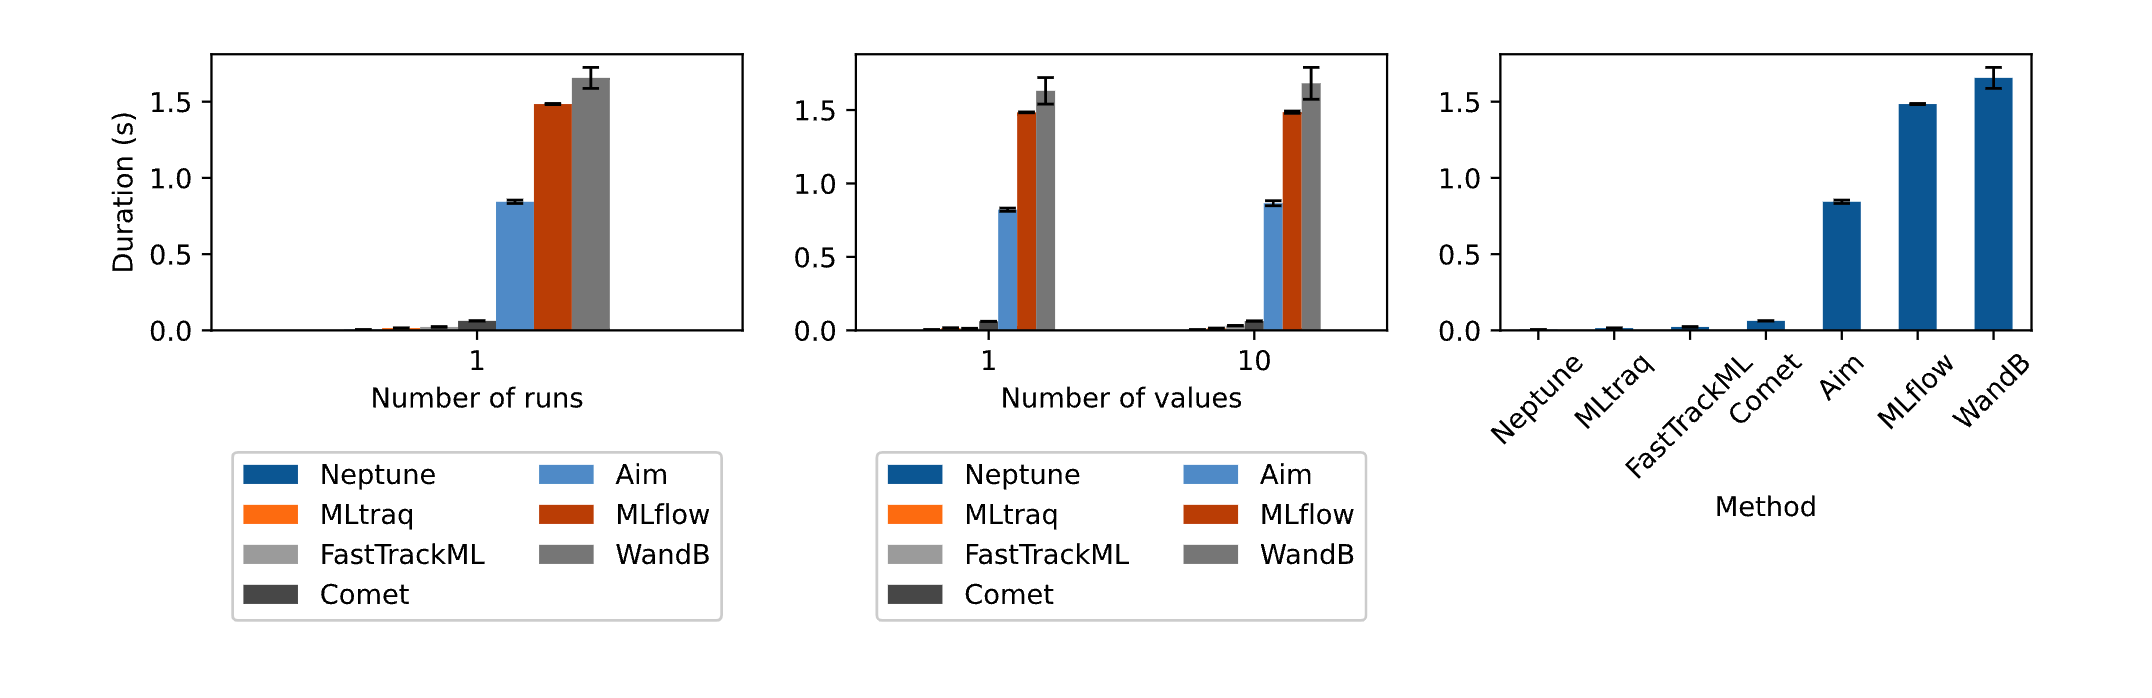
\includegraphics[width=\textwidth]{images/mltraq/mltraq-Initialization-time.png}
    \caption{Initialization time for tracking a single value across different experiment tracking solutions.}
    \label{fig:init-time}
\end{figure}

The results, shown in Figure \ref{fig:init-time}, indicate the following:

\begin{itemize}
    \item \textbf{W\&B and MLflow:} These tools perform the worst due to threading and event management, costing up to 400 times more than the other methods.
    \item \textbf{Aim:} Spends most of the time creating and managing its embedded key-value store.
    \item \textbf{Comet:} The cost is primarily due to thread management.
    \item \textbf{FastTrackML:} Remarkably fast in creating new runs due to its background server, which eliminates most of the database initialization cost.
    \item \textbf{MLtraq:} Writing to SQLite is the primary cost.
    \item \textbf{Neptune:} Performs best with no threading, no SQLite database, and simply writing the tracking data to files.\newline
\end{itemize}

\textbf{Experiment 2: High-Frequency Tracking}

While efficient initialization is essential, the ability to monitor many values quickly is critical for any tracking solution. This experiment assesses the time required to track and store up to 10,000 values.

\begin{figure}[h!]
    \centering
    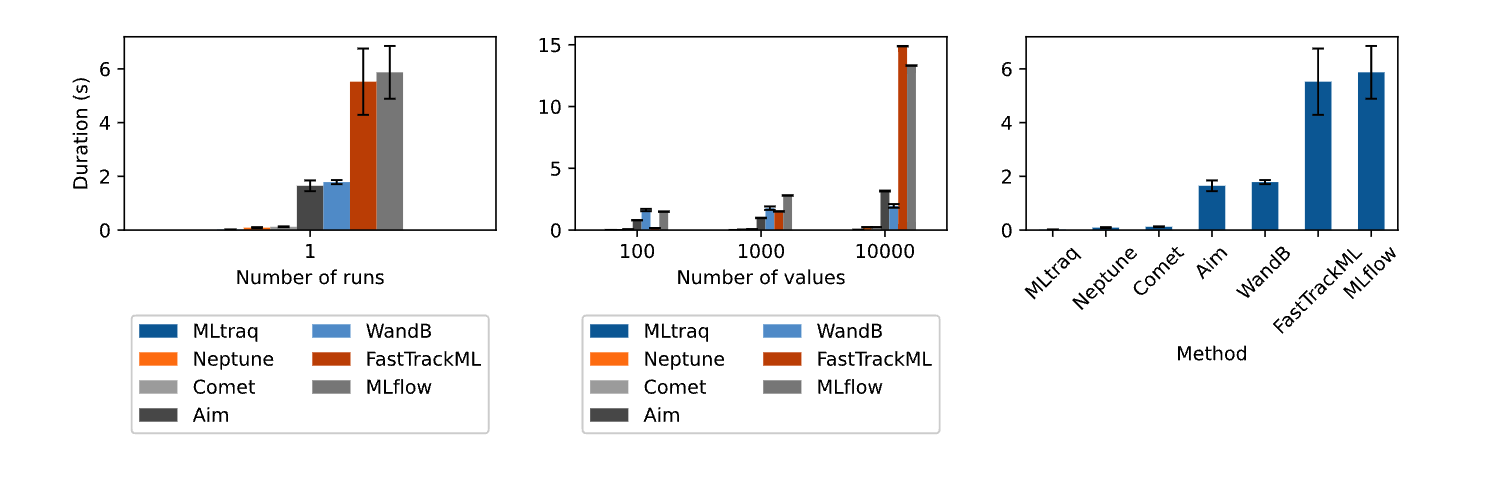
\includegraphics[width=\textwidth]{images/mltraq/mltraq-high-frequency.png}
    \caption{High-frequency tracking performance for up to 10,000 values across different experiment tracking solutions.}
    \label{fig:high-freq}
\end{figure}

The results, illustrated in Figure \ref{fig:high-freq}, highlight the following:

\begin{itemize}
    \item \textbf{FastTrackML:} While efficient in creating new runs, inserting new tracking records is similarly expensive to MLflow due to their entity-attribute-value database model.
    \item \textbf{Aim and W\&B:} Perform at a fraction of the cost compared to MLflow and FastTrackML.
    \item \textbf{Neptune, Comet, and MLtraq:} These are the highest-performing methods, with MLtraq being the fastest, up to 100 times faster than W\&B.\newline
\end{itemize}

\subsubsection{Key Features}

MLtraq includes a range of features designed to enhance the experiment tracking process:

\begin{itemize}
    \item \textbf{Immediate:} Allows the design and execution of experiments with just a few lines of code and supports metric streaming.
    \item \textbf{Collaborative:} Supports backing up, merging, sharing, and reloading experiments with their computation state anywhere.
    \item \textbf{Interoperable:} Provides access to experiments through Python, Pandas, and SQL with native database types and open formats.
    \item \textbf{Flexible:} Tracks native Python data types and structures, as well as NumPy, Pandas, and PyArrow objects.
    \item \textbf{Lightweight:} A thin layer with minimal dependencies that can run anywhere and complement other components and services.
\end{itemize}

\subsubsection{Design Choices}

MLtraq incorporates several thoughtful design choices to optimize its functionality:

\begin{itemize}
    \item \textbf{Computation:} Uses joblib.Parallel for process-based parallelism in chained execution of steps. It also supports cluster-specific backends like Dask, Ray, and Spark, requiring step functions and run objects to be serializable with cloudpickle.
    \item \textbf{Persistence:} Defaults to SQLite but can connect to any SQL database supported by SQLAlchemy. It supports a wide range of data types and provides a Data store interface for handling large objects. Compression is available but disabled by default.
\end{itemize}

In summary, MLtraq stands out as a powerful and efficient tool for tracking ML and AI experiments. It outperforms other solutions in terms of initialization time and high-frequency tracking performance, demonstrating significant advantages in speed, flexibility, and ability to handle complex data structures. Its unique features, such as the DATAPAK format for serialization, flexible storage options, and robust support for collaborative efforts, make it an invaluable resource for developers. Careful design choices further enhance its functionality, making MLtraq the optimal choice for scalable and efficient tracking of experiments. Delving deeper into the analysis of this innovative approach, it becomes clear that MLtraq offers unparalleled performance and reliability, setting a new standard in the field of experiment tracking.

\newpage

\section{State-of-the-art Models}
Selection of state-of-the-art LLMs (GPT-4o, Claude 3.5, Gemini Pro, Mistral, Meta Llama 3,...) to compare their differences in performance, architecture, accessibility and cost for developing question-answering chatbot systems.

\subsection{Challenges and Limitations}
Discussion on cost, carbon footprint and energy consumption and privacy concerns.

\subsection{Beyond Transformers: the Mamba LLM Architecture}
Discover the power of Mamba LLM, a transformative architecture from leading universities, redefining sequence processing in AI.

